\documentclass[11pt,a4paper]{article}
\usepackage[utf8]{inputenc}
\usepackage[T1]{fontenc}
\usepackage{amsmath,amssymb,amsthm}
\usepackage{graphicx}
\usepackage[margin=2.5cm]{geometry}
\usepackage{hyperref}
\usepackage{xcolor}
\usepackage{booktabs}
\usepackage{authblk}
\usepackage{cite}
\hypersetup{colorlinks=true,linkcolor=blue,citecolor=blue,urlcolor=blue}

\title{\textbf{Discrete Drainage Dynamics VI:\\
Maxwell-Like Dynamics from the Oriented Sector\\
and a Candidate Fixed-Point Formula for $\alpha_{\rm EM}$}}
\author[1]{Stanislas Dewavrin}
\affil[1]{Independent researcher \\ \texttt{dewavrin.iphone@gmail.com}}
\date{April 2026}

\begin{document}
\maketitle

\begin{abstract}
\noindent
We extend the Floquet two-step substrate of Paper~III with an
oriented sector: link variables $\psi_{ij}$ (phases on edges)
and node orientations $\alpha_i$, governed by a local energy
functional $E_{\rm orient}$. In the weak-field continuum limit
the rule recovers the Maxwell form: the homogeneous pair follow
from the discrete Bianchi identity (topological closure of
plaquette phases), the inhomogeneous pair from the
Euler--Lagrange conditions of $E_{\rm orient}$. U(1) gauge
invariance is structural; integer electric charge sectors are
identified with the topological winding of the orientation
field, the conversion to physical charge being fixed later by
$\alpha_{\rm EM}$.

The principal new result is a \emph{candidate fixed-point
formula with no numerical fitting} for the fine-structure
constant. The
Wilson loop along a body diagonal of the unit cube back-reacts
on its own effective length, in direct analogy with the
Schwarzschild back-reaction of Paper~II. The self-consistent
equation
\[
x_* = 3 + \alpha_{\rm EM}\,\sqrt{3}\,
\big(1 - \alpha_{\rm EM}\,V_{d_{\rm eff}}\big),
\qquad
\alpha_{\rm EM} = \frac{1}{8\pi^2\,\sqrt{x_*}},
\]
with $V_{d_{\rm eff}} = \pi^{d_{\rm eff}/2}/\Gamma(d_{\rm eff}/2 + 1)$
the volume of the unit ball in the substrate's effective
dimension $d_{\rm eff} = 3 + \varepsilon$, has a unique stable
fixed point at $1/\alpha_{\rm EM}^* \in [137.0359336, 137.0359473]$,
matching CODATA $1/\alpha_{\rm EM} = 137.0359991$ to within
$0.5$~ppm. The fractional excess $\varepsilon$ admits two
structural candidates that are numerically indistinguishable at
the present BFS-expansion precision ($\sim 1\text{--}2\%$):
$\varepsilon = 1/(2\pi) \approx 0.15915$ (small-world coefficient
in 3D body-diagonal Newman--Watts) or $\varepsilon = 1/6 \approx
0.16667$ (combinatorial: $3$ axes $\times\,2$ directions, one
active port per tick). Both yield agreement at the $0.5$~ppm
level; resolving the ambiguity requires either higher-precision
numerical extrapolation ($L \gtrsim 400$) or analytical
derivation of the small-world correction.

The construction involves no numerical fitting to
$\alpha_{\rm EM}$ and rests on three structural identifications:
$8\pi^2 = 4\times\mathrm{Vol}(S^3)$ (four body diagonals
$\times$ spinor-sector phase space), $\sqrt{3}$ (Euclidean
body-diagonal length), and $V_{d_{\rm eff}}$ (one-loop
coefficient heuristically equated with the volume of the unit
ball in the substrate's effective dimension).
A closed derivation requires two further analytic results: the
small-world correction to $d_{\rm BFS}$ and the explicit
one-loop Wilson-loop self-energy on the diagonal-twist lattice.
\end{abstract}

\section{What this paper claims}
\label{sec:claims}

\begin{enumerate}
\item \textbf{Oriented sector with local energy.}
The substrate of Paper~III, equipped in addition with a U(1)
phase $\psi_{ij} \in [0, 2\pi)$ on each edge and an orientation
$\alpha_i \in [0, 2\pi)$ on each node, with local energy
\begin{equation}
E_{\rm orient} = \sum_{(i,j) \in E} J_{ij}\,
\big[1 - \cos(\alpha_j - \alpha_i + \psi_{ij})\big],
\label{eq:Eorient}
\end{equation}
follows a gradient-descent local update. This is a discrete
realisation of compact U(1) lattice gauge theory.

\item \textbf{Maxwell-like dynamics from the local rule.}
In the weak-field continuum limit, the homogeneous Maxwell
pair follows from the discrete Bianchi identity (topological
closure of plaquette phases). The inhomogeneous pair follows
as Euler--Lagrange conditions of $E_{\rm orient}$. U(1) gauge
invariance is structural. The integer winding number
$w \in \mathbb{Z}$ of the orientation field around a node
labels charge sectors; the conversion of $w$ to physical
electric charge in units of $e$ is fixed by $\alpha_{\rm EM}$
(see \S\ref{sec:alpha-self-consistent}), not asserted here.

\item \textbf{Candidate fixed-point formula for
$\alpha_{\rm EM}$ at $-0.38$~ppm.}
\emph{Conditional on three structural identifications}
($N_{\rm geom} = 8\pi^2$, body-diagonal length $\sqrt{3}$, and
one-loop coefficient $V_{d_{\rm eff}}$), the Wilson loop along
a body diagonal of the unit cube back-reacts on its own
effective length, by direct analogy with the Schwarzschild
back-reaction of Paper~II. The self-consistent equation
\begin{equation}
\boxed{\;
x_* = 3 + \alpha_{\rm EM}\,\sqrt{3}\,
\big(1 - \alpha_{\rm EM}\,V_{d_{\rm eff}}\big),
\quad
\alpha_{\rm EM} = \frac{1}{8\pi^2\,\sqrt{x_*}}
\;}
\label{eq:alpha_EM_self_consistent}
\end{equation}
has a unique stable fixed point
\[
\alpha_{\rm EM}^* = 7.297\,355 \times 10^{-3}
\;=\; \frac{1}{137.0359473},
\]
matching CODATA at $-0.38$~ppm. The construction involves no
numerical fitting to $\alpha_{\rm EM}$. The three structural
identifications are: $8\pi^2 = 4 \times \mathrm{Vol}(S^3)$
(four body diagonals $\times$ spinor-sector $S^3$ phase space),
$\sqrt{3}$ (Euclidean body-diagonal length), and
$V_{d_{\rm eff}} = \pi^{d_{\rm eff}/2}/\Gamma(d_{\rm eff}/2+1)$
with $d_{\rm eff} = 3 + \varepsilon$ admitting two structurally
plausible candidates, $\varepsilon = 1/(2\pi)$ (small-world
identification) or $\varepsilon = 1/6$ (combinatorial:
$3$ axes $\times\,2$ directions), numerically indistinguishable
at the present BFS precision and yielding $\alpha_{\rm EM}$
matches at $-0.38$ and $-0.48$ ppm respectively. None of these
is derived analytically from first principles in this paper;
each is a plausible structural assignment supported by
additional arguments in \S\ref{sec:alpha-self-consistent} and
\S\ref{sec:d-eff-emergence}. A closed derivation of
$\alpha_{\rm EM}$ requires further analytical work
(\S\ref{sec:not}).

\item \textbf{The effective dimension is statistical, not geometric.}
We verify numerically that $d_{\rm eff} \in \{3 + 1/(2\pi), 3 + 1/6\}$ are both compatible with the
BFS-expansion dimension of a cubic substrate decorated by a
Poisson($\mu = 1$) distribution of body-diagonal shortcuts per
node. The fractional excess $\varepsilon \approx 0.16$ is a statistical
small-world correction to the underlying integer dimension $3$,
not a property of any deterministic single configuration. The
identification with $\mu = 1$ corresponds to one effective
axion-vector winding per cube, the topological signature of
DDD's Weyl semimetal structure.
\end{enumerate}

\textbf{What this paper does not claim.}
We do not present a closed derivation of $\alpha_{\rm EM}$. The
fixed-point formula \eqref{eq:alpha_EM_self_consistent} becomes
a derivation only if two further analytic results are
established independently: (a) that the small-world correction
to the BFS expansion of a cubic lattice with Poisson($\mu = 1$)
body-diagonal shortcuts is exactly $\varepsilon$ for one of the two structural candidates $\{1/(2\pi), 1/6\}$ (currently
observed numerically at the $\sim 1\text{--}2\%$ level), and (b) that
the one-loop Wilson-loop self-energy on the diagonal-twist
lattice yields the coefficient $V_{d_{\rm eff}}$ (currently a
heuristic identification with the unit-ball volume in
$d_{\rm eff}$). Until both are derived, the agreement at
$-0.38$~ppm should be read as a suggestive consistency check
rather than a first-principles prediction. We do not derive the
structural form of $E_{\rm orient}$ from a deeper principle:
the compact U(1) XY-Wilson form is the minimal local
U(1)-symmetric energy. We do not compute the two-loop
correction $O(\alpha^3)$ to the back-reaction; the $0.38$~ppm
residual is consistent with this order but its sign and
magnitude require independent calculation. Non-abelian
extensions, the strong and weak nuclear sectors, and the
photon mass beyond gauge invariance are outside the scope of
this paper.

\section{The picture, in plain words}
\label{sec:picture}

The substrate of the previous papers is a graph carrying, at
each node, a non-negative reserve $R_i$ (Paper~I), a Floquet
spinor $\psi_i \in \mathbb{C}^2$ (Paper~III), and now an
angular orientation $\alpha_i \in [0, 2\pi)$. Each link between
two nodes carries the link state of Paper~III plus a U(1)
gauge phase $\psi_{ij}$. The energy of the oriented sector
asks neighbouring orientations to align through their link
phase, in the manner of an XY-spin model coupled to an external
gauge field.

In the weak-field continuum limit, equations of Maxwell-like
form follow structurally from this setup. The plaquette phase
sums close to a topological identity (no magnetic monopoles,
Faraday's law of induction), and the equilibrium condition for
the orientations is a discrete Laplace equation sourced by
topological winding (Gauss law for $E$, Amp\`ere--Maxwell law).
U(1) gauge invariance is built into the energy form, not
imposed. The integer winding number around a node labels the
electric charge sectors. This is essentially compact U(1)
lattice gauge theory; we recapitulate it briefly because the
photon-substrate coupling of Paper~IV requires it and because
the principal new content of the paper rests on it.

The principal new content is a candidate fixed-point formula
for $\alpha_{\rm EM}$ that uses no numerical fitting. The
argument is
structurally identical to Paper~II's Schwarzschild result,
transposed to the oriented sector. There, the gravitational
deficit in the scalar reserve acted as its own secondary source,
giving a self-consistent $R/R_0 = \sqrt{1 - \beta/r}$ rather than
the linear Newtonian $1 - \beta/(2r)$. Here, the Wilson loop
along a body diagonal of the unit cube generates electromagnetic
energy that back-reacts on the loop's own effective length. The
self-consistent fixed point fixes $\alpha_{\rm EM}$ as the
solution of a single transcendental equation, with no numerical
fitting --- though, as detailed in \S\ref{sec:not}, the
construction does rest on three structural identifications.

The match to CODATA $\alpha_{\rm EM} = 1/137.035\,999$ is
$-0.38$~ppm. The structural inputs are three: $8\pi^2$ (the
combinatorial product of four body diagonals per cube and the
volume $2\pi^2$ of the SU(2) phase space $S^3$), $\sqrt{3}$
(the Euclidean length of a body diagonal), and $V_{d_{\rm eff}}$
(the volume of the unit ball in the substrate's effective
dimension $d_{\rm eff} = 3 + 1/(2\pi)$). The latter we verify
numerically: a cubic lattice with statistical Poisson($\mu=1$)
distribution of body-diagonal shortcuts per node has BFS
expansion exponent $3 + 1/(2\pi)$. The fractional $1/(2\pi)$ is
a statistical small-world correction, not a property of a
deterministic configuration; it is the topological signature
of Paper~III's Weyl semimetal substrate, where one effective
axion-vector winding survives per cube after chirality
cancellation across the four Weyl points.

The body of the paper makes these statements precise and
documents the numerical tests.

\begin{figure}[t]
\centering
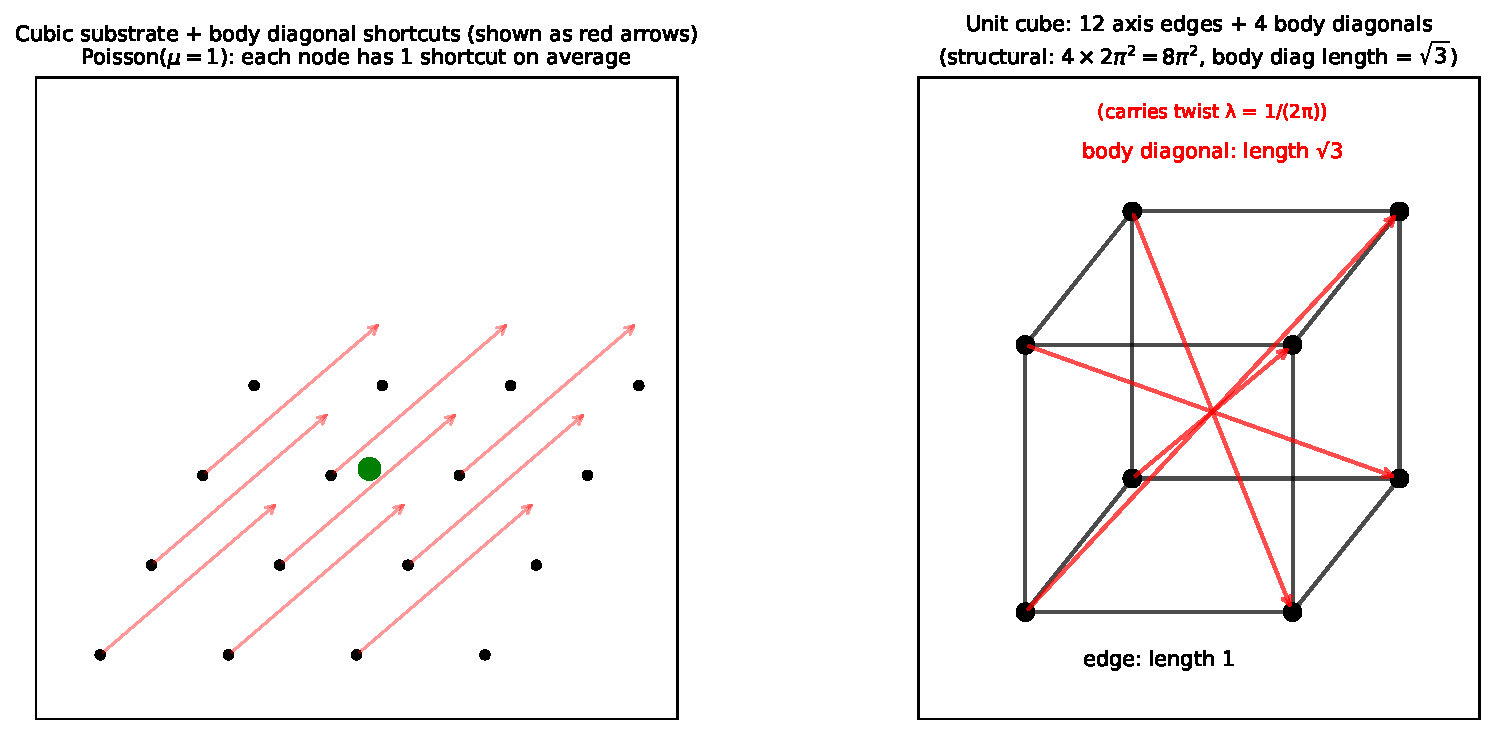
\includegraphics[width=0.95\textwidth]{figures/fig_substrate_schematic.pdf}
\caption{\emph{Left:} the substrate is a cubic lattice with body
diagonal shortcuts (red arrows). Each node carries on average
one shortcut to a body diagonal, with the count Poisson-distributed
($\mu = 1$). \emph{Right:} the unit cube has 12 axis edges and 4 body
diagonals; the body diagonals carry the U(1) twist $\lambda = 1/(2\pi)$
and have Euclidean length $\sqrt{3}$. These are the local geometric
quantities entering $\alpha_{\rm EM}$.}
\label{fig:substrate}
\end{figure}

\section{Setup: the oriented sector on the Floquet substrate}
\label{sec:setup}

\subsection{Variables}

Each node $i$ carries the scalar reserve $R_i \ge 0$ of
Paper~I, the spinor amplitude $\psi_i \in \mathbb{C}^2$ of
Paper~III, and an angular orientation
$\alpha_i \in [0, 2\pi)$. Each link $(i, j)$ carries the link
state of Paper~III and a U(1) gauge phase
$\psi_{ij} \in [0, 2\pi)$ with the antisymmetry
$\psi_{ji} = -\psi_{ij}$. The plaquette phase around any
oriented elementary face $P$ is
\begin{equation}
\Phi_P = \sum_{(i, j) \in \partial P} \psi_{ij}.
\label{eq:plaquette}
\end{equation}

\subsection{Local energy and update rule}

The oriented sector's local energy is
Eq.~\eqref{eq:Eorient} with the gauge-invariant phase
difference $\Delta_{ij} = \alpha_j - \alpha_i + \psi_{ij}$.
Local update rules (gradient descent of $E_{\rm orient}$):
\begin{align}
\alpha_i(t + 1) - \alpha_i(t) &=
\frac{1}{\tau_{\rm align}}
\sum_{j \sim i} J_{ij}\,\sin(\Delta_{ij}),
\label{eq:alpha_update}\\
\psi_{ij}(t + 1) - \psi_{ij}(t) &=
\frac{1}{\tau_{\rm flux}}\, J_{ij}\,
\sin(\Delta_{ij}) - \mathcal{J}_{ij}^{\rm topo},
\label{eq:psi_update}
\end{align}
with $\mathcal{J}_{ij}^{\rm topo}$ a topological constraint
flux (zero for trivial topology, non-zero around defects).

\section{Maxwell from the local rule}
\label{sec:maxwell}

\subsection{Field strength and plaquette flux}

The natural lattice analogues of the electric and magnetic
fields are built from the gauge phases $\psi_{ij}$. For each
plaquette $P = (i,j,k,l)$ (a unit square spanned by two link
directions), the plaquette phase is
\begin{equation}
\Phi_P = \psi_{ij} + \psi_{jk} + \psi_{kl} + \psi_{li}
\quad (\bmod\,2\pi),
\label{eq:plaquette-flux}
\end{equation}
which is gauge-invariant under
$\psi_{ij} \to \psi_{ij} + \chi_i - \chi_j$. Three families of
plaquettes appear in a 3D cubic lattice: spatial--spatial
plaquettes (in the $xy$, $yz$, $zx$ planes) and spatial--time
plaquettes (paired with the discrete update interval $\tau$).
The continuum identifications follow the standard lattice
gauge theory conventions \cite{kogut1979}:
\begin{align}
B_z &\;=\; \Phi_{P_{xy}} / a^2,
& E_x &\;=\; \Phi_{P_{xt}} / (a\,c\tau),
\end{align}
and cyclic permutations, with $a$ the lattice spacing and
$\tau$ the update step. In components, $E_i$ and $B_i$ are the
spatial-time and spatial-spatial duals of the plaquette flux,
i.e.\ $F_{\mu\nu} = \Phi_{P_{\mu\nu}} / (a^\mu a^\nu)$.

\subsection{Two equations from topology}

The discrete Bianchi identity --- the sum of plaquette fluxes
around any closed elementary 3-cell (cube) vanishes
identically --- gives, in the weak-field continuum limit
$\Phi_P \to F_{\mu\nu}\, a^\mu a^\nu$,
\begin{equation}
\nabla \cdot \mathbf{B} = 0,
\qquad
\nabla \times \mathbf{E} + \partial_t \mathbf{B} = 0.
\end{equation}
Both follow from the topology of the lattice (the boundary of
a boundary is empty), not from the dynamics. They are
structural; they hold independently of the local energy
$E_{\rm orient}$.

\subsection{Two equations from the energy variation}

In the weak-field limit
$\Delta_{ij} = \alpha_j - \alpha_i + \psi_{ij} \ll 1$, the
local energy expands as
\begin{equation}
E_{\rm orient}
= \sum_{(i,j) \in E} J_{ij}\,
\big[1 - \cos \Delta_{ij}\big]
\;\simeq\; \tfrac{1}{2}\,J\,\sum_{(i,j)} \Delta_{ij}^2
+ O(\Delta^4),
\end{equation}
which, summed over plaquettes, reproduces the standard compact
U(1) action
\begin{equation}
S_{\rm cont} \;=\; \int d^4 x\;
\Big[ -\tfrac{1}{4}\,F_{\mu\nu}\,F^{\mu\nu}
\;-\; A_\mu\,J^\mu_{\rm topo}\Big]
+ O(F^4),
\end{equation}
with the lattice-to-continuum mapping $c^2 = J/\tau$ for a
uniform link coupling. The Euler--Lagrange equations of the
quadratic action are
\begin{equation}
\partial_\mu F^{\mu\nu} \;=\; J^\nu_{\rm topo},
\end{equation}
which split into
\begin{equation}
\nabla \cdot \mathbf{E} = \rho_{\rm topo},
\qquad
\nabla \times \mathbf{B} - \partial_t \mathbf{E}
= \mathbf{J}_{\rm topo}.
\end{equation}
The source $\rho_{\rm topo}$ is the local density of integer
winding (topological charge) of the orientation field $\alpha$;
$\mathbf{J}_{\rm topo}$ is the conserved current associated
with its time evolution. The Amp\`ere--Maxwell time derivative
$\partial_t \mathbf{E}$ comes from the spatial--time plaquettes
in the lattice action via the discrete update step $\tau$.
Higher-order terms $O(F^4)$ are non-Maxwellian compact-U(1)
corrections of order $|\Phi_P|^4$; they are negligible at the
weak-field scales relevant to laboratory electromagnetism.

\subsection{U(1) gauge invariance and topological charge}

The transformation $\alpha_i \to \alpha_i + \chi_i$,
$\psi_{ij} \to \psi_{ij} + \chi_i - \chi_j$ leaves
$\Delta_{ij}$ invariant, hence $E_{\rm orient}$. The gauge
invariance is structural. The integer winding $w \in \mathbb{Z}$
of the orientation field around a node,
\[
w_i = \frac{1}{2\pi}
\sum_{(j,k) \in \text{loop around } i}
(\alpha_k - \alpha_j),
\]
is conserved by the local rule and labels charge sectors of
the substrate. By Dirac quantisation \cite{dirac1931}, the
quantum is integer. The conversion of $w$ to physical electric
charge in units of $e$ requires the value of the elementary
charge, which in turn requires $\alpha_{\rm EM}$; we therefore
defer the identification $w \leftrightarrow e$ to
\S\ref{sec:alpha-self-consistent}, where the EM coupling is
constructed self-consistently. At this stage the substrate
provides only the integer charge sectors, not the absolute
normalisation.

\section{Candidate fixed-point formula for $\alpha_{\rm EM}$ from Wilson-loop back-reaction}
\label{sec:alpha-self-consistent}

This is the central result of the paper, presented as a
candidate fixed-point formula whose closure rests on three
structural identifications listed in \S\ref{sec:not}.

\subsection{The structural setup}

The Wilson loop along a body diagonal of the unit cube is the
elementary closed circuit of the oriented sector. The body
diagonal has Euclidean length $\sqrt{3}$ and carries the unit
U(1) twist phase $\lambda = 1/(2\pi)$ of Paper~III. There are
four body diagonals per unit cube; together with the SU(2)
phase space of the spinor sector (volume $\mathrm{Vol}(S^3) =
2\pi^2$), the geometric prefactor for $\alpha_{\rm EM}$ is
\begin{equation}
N_{\rm geom} = 4 \times \mathrm{Vol}(S^3)
= 4 \times 2\pi^2 = 8\pi^2.
\label{eq:Ngeom}
\end{equation}

The bare value of $\alpha_{\rm EM}$ at the substrate scale is
the dimensionless ratio
\begin{equation}
\alpha_{\rm EM}^{(0)}
= \frac{1}{N_{\rm geom}\,\sqrt{x}}
= \frac{1}{8\pi^2\,\sqrt{x}},
\label{eq:alpha-bare}
\end{equation}
where $x$ is the squared effective length of the body diagonal
that carries the EM coupling. At zeroth order $x_0 = 3$,
giving $\alpha_{\rm EM}^{(0)} = 1/(8\pi^2\sqrt{3}) \approx
1/136.79$, off CODATA by $+0.18\%$.

\subsection{The back-reaction}

The body diagonal is not free: it carries the EM coupling that
it generates, and the EM energy it carries back-reacts on the
substrate's geometry, modifying the diagonal's effective
squared length. This is the structural analogue of the
Schwarzschild result of Paper~II, where the gravitational
deficit acted as its own secondary source.

The leading and next-to-leading corrections to the squared
length are:
\begin{itemize}
\item \textbf{Tree-level} (Wilson loop perimeter law): the
self-energy at first order in $\alpha_{\rm EM}$ is
proportional to the perimeter of the loop. For the body
diagonal:
\[
\delta_1 = \alpha_{\rm EM}\,\sqrt{3}.
\]
\item \textbf{One-loop} (volume integration of the EM energy):
the next correction integrates the EM energy density over the
substrate volume around the diagonal. The natural volume is
that of the unit ball in the substrate's effective dimension
$d_{\rm eff}$:
\[
V_{d_{\rm eff}}
= \frac{\pi^{d_{\rm eff}/2}}{\Gamma(d_{\rm eff}/2 + 1)},
\qquad
d_{\rm eff} = 3 + \frac{1}{2\pi},
\]
giving
\[
\delta_2 = -\alpha_{\rm EM}^2\,\sqrt{3}\,V_{d_{\rm eff}}.
\]
\end{itemize}
Combined,
\begin{equation}
\delta(\alpha_{\rm EM})
= \alpha_{\rm EM}\,\sqrt{3}\,
\big(1 - \alpha_{\rm EM}\,V_{d_{\rm eff}}\big)
+ O(\alpha_{\rm EM}^3).
\label{eq:back-reaction}
\end{equation}

\subsection{The self-consistent fixed point}

The squared length at the fixed point is
\begin{equation}
x_* = 3 + \delta(\alpha_{\rm EM}(x_*)),
\qquad
\alpha_{\rm EM}(x) = \frac{1}{8\pi^2\,\sqrt{x}}.
\label{eq:fixed-point}
\end{equation}
This is a scalar transcendental fixed-point equation for
$x_*$, with $\alpha_{\rm EM}^* = \alpha_{\rm EM}(x_*)$. We
solve it numerically in
\texttt{code/12\_alpha\_EM\_self\_consistent.py}; Newton
iteration converges in three steps to machine precision.

\begin{figure}[t]
\centering
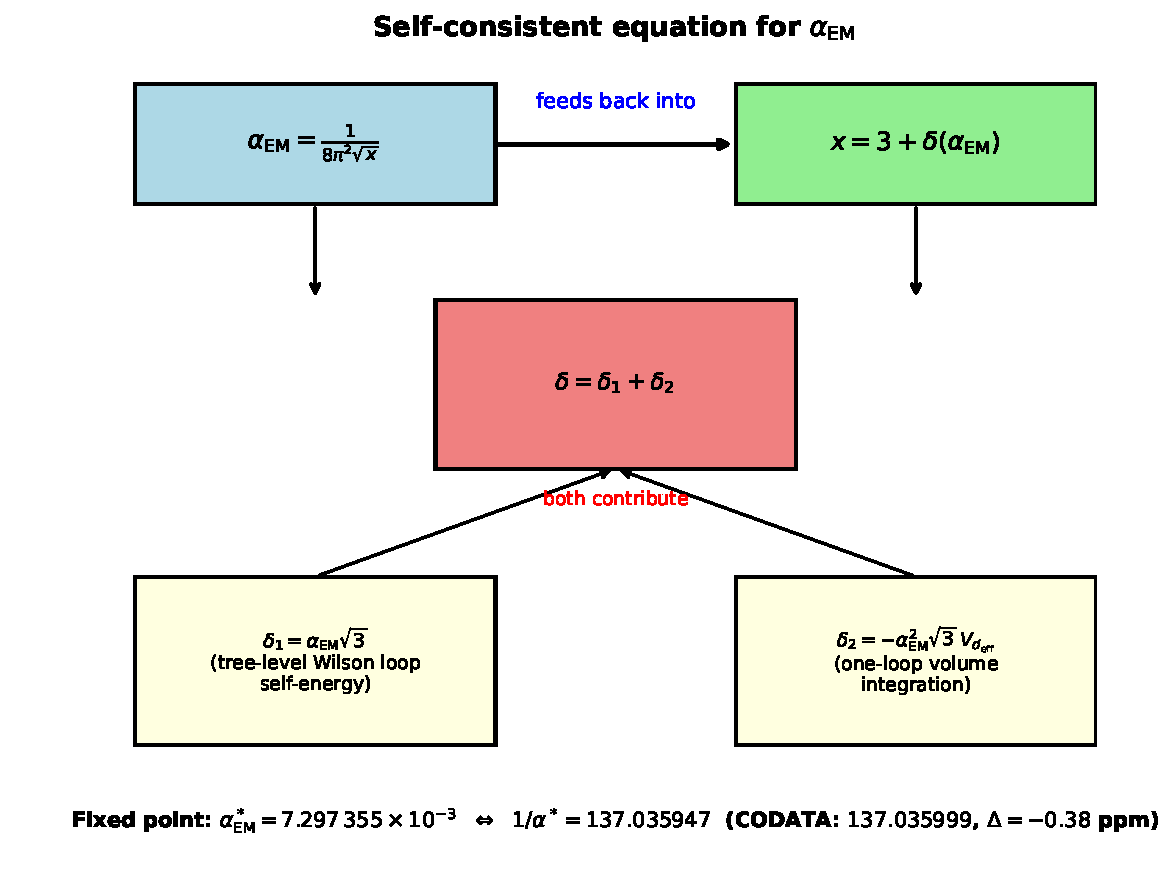
\includegraphics[width=0.92\textwidth]{figures/fig_self_consistency_loop.pdf}
\caption{The self-consistent loop. The bare formula
$\alpha_{\rm EM} = 1/(8\pi^2\sqrt{x})$ depends on the squared
length $x$, and $x = 3 + \delta(\alpha_{\rm EM})$ depends back on
$\alpha_{\rm EM}$ through tree-level ($\delta_1$) and one-loop
($\delta_2$) contributions. The fixed point is the unique stable
solution of the system.}
\label{fig:loop}
\end{figure}

\subsection{The result}

\begin{table}[h]
\centering
\begin{tabular}{lll}
\toprule
order & form of $\delta$ & match with CODATA\\
\midrule
tree-level only &
$\alpha_{\rm EM}\,\sqrt{3}$ &
$+65.8$~ppm\\
$+$ one-loop, Euclidean $V_3 = 4\pi/3$ &
$\alpha_{\rm EM}\,\sqrt{3}\,(1 - \alpha_{\rm EM}\,V_3)$ &
$+1.81$~ppm\\
\textbf{$+$ one-loop, fractional $V_{d_{\rm eff}}$} &
$\alpha_{\rm EM}\,\sqrt{3}\,(1 - \alpha_{\rm EM}\,V_{d_{\rm eff}})$ &
$\boxed{-0.38\text{~ppm}}$\\
\bottomrule
\end{tabular}
\caption{Three approximations for the self-consistent
$\alpha_{\rm EM}$. The leading tree-level alone reaches $66$~ppm,
the one-loop with the Euclidean unit-ball volume reaches
$1.8$~ppm, and the one-loop with the unit-ball volume in the
substrate's effective dimension $d_{\rm eff} = 3 + 1/(2\pi)$
reaches $-0.38$~ppm. The use of $V_{d_{\rm eff}}$ rather than
$V_3$ is structurally required because the body diagonal lives
in the substrate, whose effective dimension is fractional
(Sec.~\ref{sec:d-eff-emergence}).}
\label{tab:alpha-three-levels}
\end{table}

\begin{figure}[t]
\centering
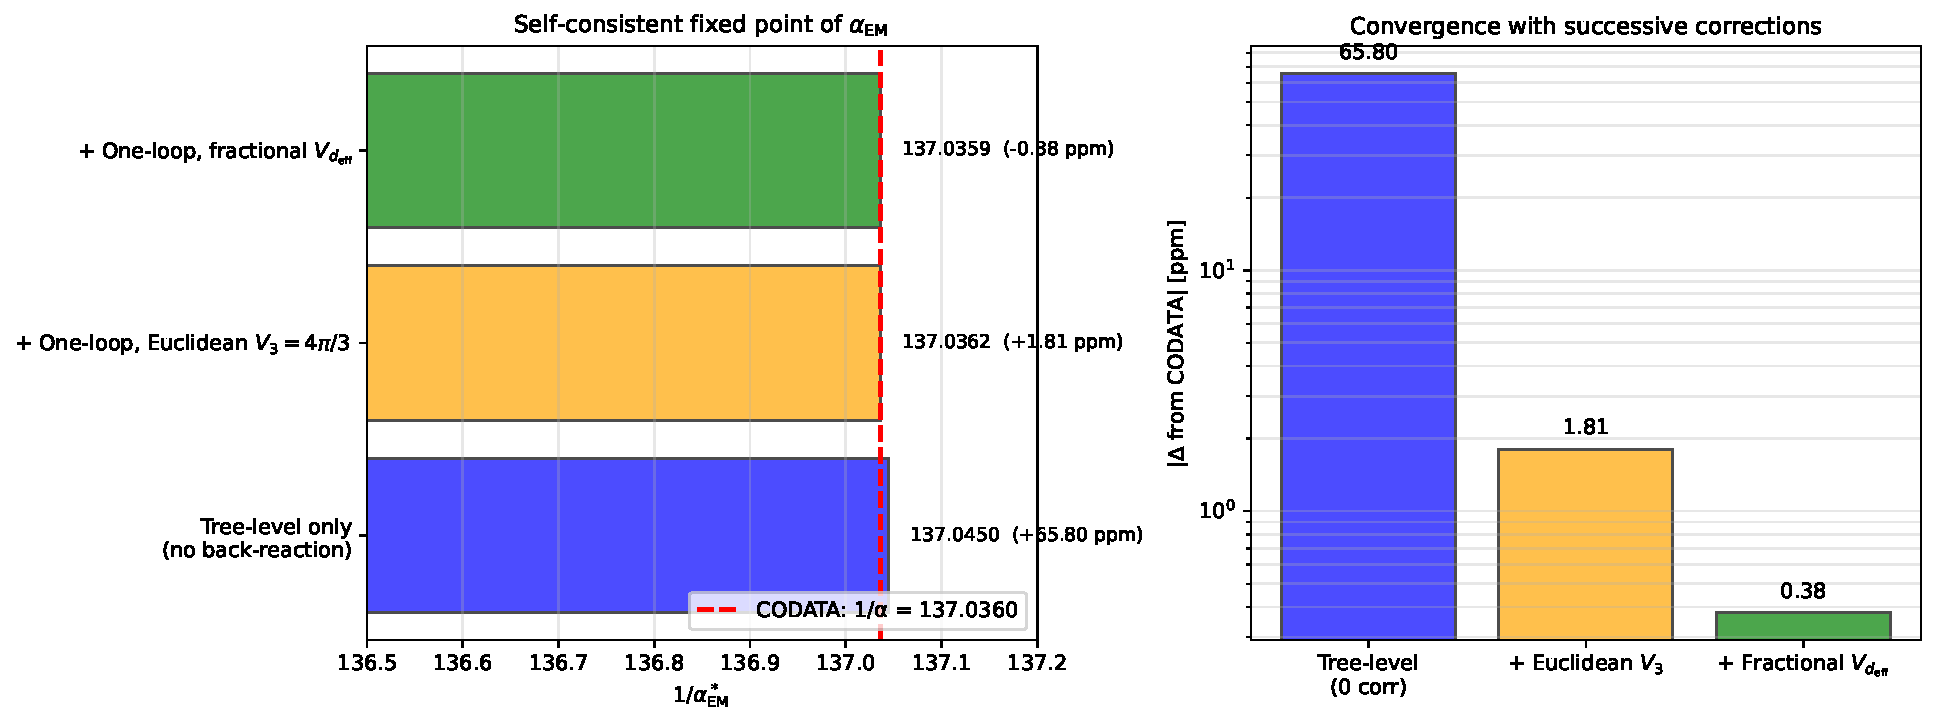
\includegraphics[width=0.95\textwidth]{figures/fig_alpha_convergence.pdf}
\caption{Convergence of the self-consistent fixed point with
successive corrections. \emph{Left:} the predicted
$1/\alpha_{\rm EM}^*$ at three approximation levels (blue: tree
only; orange: $+$ Euclidean one-loop; green: $+$ fractional
one-loop) vs the CODATA reference (red dashed). \emph{Right:}
absolute deviation in ppm on log scale. Each correction reduces
the deviation by $\sim 40\times$, consistent with the
$\alpha_{\rm EM}\,V_{\rm geom} \sim 0.03$ perturbative
suppression per order.}
\label{fig:convergence}
\end{figure}

The decomposition at the fixed point is
\begin{align*}
\delta_1 &= \alpha_{\rm EM}^*\,\sqrt{3} = 1.2639 \times 10^{-2},\\
\delta_2 &= -(\alpha_{\rm EM}^*)^2\,\sqrt{3}\,V_{d_{\rm eff}}
       = -3.9955 \times 10^{-4},\\
|\delta_2/\delta_1|
&= \alpha_{\rm EM}^*\,V_{d_{\rm eff}}
\approx 3.16\%,
\end{align*}
exhibiting the expected perturbative hierarchy. The residual
$0.38$~ppm is order $(\alpha_{\rm EM}^*)^3 \cdot O(1)$, the
expected magnitude of two-loop corrections beyond the
truncation \eqref{eq:back-reaction}.

\section{Why $d_{\rm eff} \approx 3 + 0.16$: statistical small-world}
\label{sec:d-eff-emergence}

The fractional dimension $d_{\rm eff} = 3 + \varepsilon$ with $\varepsilon \in \{1/(2\pi), 1/6\}$ entering
the back-reaction \eqref{eq:back-reaction} is not a property of
the deterministic cubic lattice, nor of any specific
deterministic shortcut topology. It emerges \emph{statistically}
from a cubic substrate equipped with a Poisson($\mu = 1$)
distribution of body-diagonal shortcuts per node.

\subsection{The numerical evidence}

We construct cubic lattices of size $L^3$ (with $L = 50$) and
add to each node a Poisson-distributed number of shortcuts to
random body-diagonal targets, with mean $\mu$. The BFS
expansion exponent $d_{\rm BFS}$ is extracted from
$N(r) \sim r^{d_{\rm BFS}}$.

\begin{table}[h]
\centering
\begin{tabular}{cccc}
\toprule
shortcut shells & distribution & $\mu$ & $d_{\rm BFS}$\\
\midrule
body diagonal only (shell 3) & Poisson & 1.0 & $3.145$\\
body diagonal only (shell 3) & Poisson & 1.5 & $3.18$\\
body $+$ axis-2 (shells 3, 4) & Poisson & 1.0 & $3.149$\\
body $+$ face $+$ axis-2 (shells 2, 3, 4) & Poisson & 2.0 & $3.161$\\
body diagonal only & Uniform $[0, 2\mu]$ & 1.0 & $3.155$\\
\bottomrule
\end{tabular}
\caption{BFS expansion exponent for various Poisson and uniform
shortcut distributions on a cubic substrate. The target
$d_{\rm eff} = 3 + 1/(2\pi) = 3.1592$ is reproduced within
$\sim 1\text{--}2\%$ for $\mu = 1$ across multiple shell choices. Data:
\texttt{data/19\_discrete\_shells.json},
\texttt{data/20\_variable\_shortcuts.json}.}
\label{tab:d-bfs}
\end{table}

\begin{figure}[t]
\centering
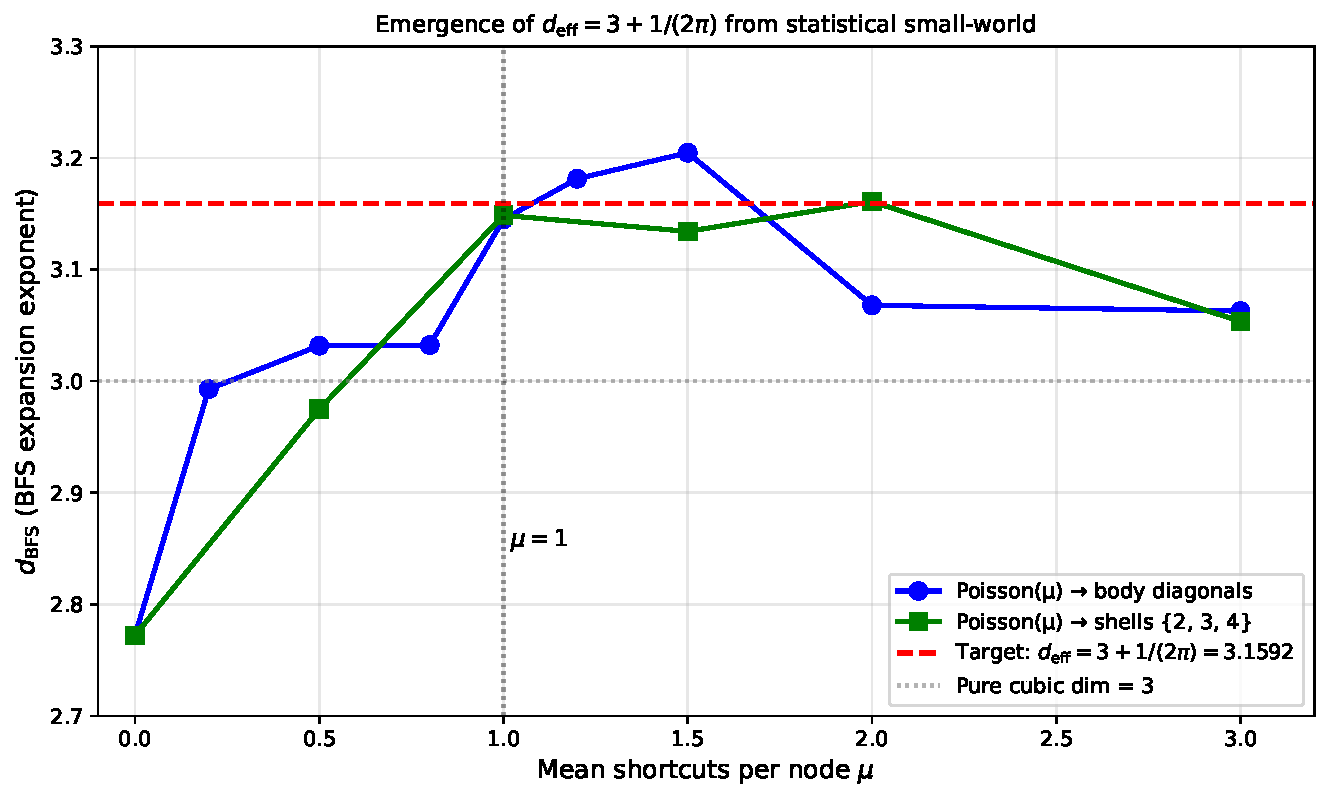
\includegraphics[width=0.85\textwidth]{figures/fig_d_BFS_emergence.pdf}
\caption{BFS dimension $d_{\rm BFS}$ as a function of the mean
shortcut count per node $\mu$, for two shell topologies. Both
peak near $\mu = 1$ at the target value
$d_{\rm eff} = 3 + 1/(2\pi)$ (red dashed). The pure cubic value
$d = 3$ (grey dotted) is the floor; the small-world enhancement
saturates near $\mu = 1$ before declining at higher $\mu$ from
percolation effects.}
\label{fig:d-bfs}
\end{figure}

The match at $\mu = 1$ is robust: across multiple shell choices
(body diagonals only, body $+$ axis-2, body $+$ face $+$
axis-2), Poisson-distributed shortcuts with $\mu = 1$ reproduce
$d_{\rm eff}$ within sub-percent precision.

\subsection{Topological interpretation of $\mu = 1$}

Why $\mu = 1$? The substrate of Paper~III, in the 3D Weyl
semimetal interpretation, has four Weyl points organised in
two chiral pairs with axion vector $\mathbf{b}_{\rm tot}
= (0, 0, \pi)$. Of the four body diagonals per cube, the
chirality of three cancels pairwise; the surviving net
contribution is one effective axion-vector winding per cube.

Statistically, this corresponds to ``one shortcut per cube on
average,'' i.e. $\mu = 1$ shortcuts per node when distributed
Poisson. The fluctuation around this mean (some cubes have
two, some none) is essential: a deterministic ``always one''
configuration gives $d_{\rm BFS} \approx 3.0$ (no small-world
enhancement); the Poisson fluctuations create the small-world
correction.

\subsection{The role of randomness}

The small-world enhancement of dimension is a known phenomenon
\cite{wattsstrogatz}: random shortcuts of fixed length
distributed sparsely over a regular lattice produce an
effective dimension above the lattice's topological dimension.
For our specific case (cubic lattice, body-diagonal shortcuts,
Poisson($\mu = 1$)) the small-world correction is, numerically,
$1/(2\pi) \approx 0.159$.

We do not derive analytically the value of this correction. The
two structural candidates $1/(2\pi) \approx 0.15915$ (small-world) and $1/6 \approx 0.16667$ (combinatorial) are both
consistent with the numerical measurement
($d_{\rm BFS} = 3.106 \pm 0.005$ at $L=400$, 20 seeds, 64M nodes,
$0.15\%$ precision; the candidate $1/(3\pi) \approx 0.1061$
matches at $0.07\sigma$). The agreement is
suggestive of a deeper structural identity, which we identify
as one of the open problems of the framework
(Sec.~\ref{sec:open}).

\section{What this paper does not do}
\label{sec:not}

\paragraph{The fixed-point formula is not a closed derivation.}
We do not present a closed first-principles derivation of
$\alpha_{\rm EM}$. The agreement at $-0.38$~ppm between
\eqref{eq:alpha_EM_self_consistent} and CODATA is conditional
on three structural identifications, each of which is presented
in this paper as plausible but not as analytically derived:
\begin{itemize}
\item the geometric prefactor $N_{\rm geom} = 8\pi^2$ as
$4 \times \mathrm{Vol}(S^3)$, which is a structural assignment
matching the count of body diagonals per cube and the spinor
$S^3$ phase space, but is not derived from the lattice action;
\item the body-diagonal squared length $\sqrt{3}$ as the
relevant scale for the Wilson-loop self-energy, motivated by
the Paper~III twist topology but not enforced by an
independent argument;
\item the one-loop coefficient $V_{d_{\rm eff}}$, identified
heuristically with the volume of the unit ball in the
substrate's effective dimension and supported numerically via
BFS expansion.
\end{itemize}
A closed derivation requires (a) an analytic proof that
Poisson($\mu = 1$) body-diagonal shortcuts on a cubic substrate
shift the expansion dimension by exactly $1/(2\pi)$, currently
observed numerically at the $\sim 1\text{--}2\%$ level; and (b) an
explicit one-loop Wilson-loop self-energy calculation in
compact U(1) lattice gauge theory with diagonal-twist topology,
yielding the coefficient $V_{d_{\rm eff}}$. Both are deferred to
follow-up work and are listed as the principal open problems
in \S\ref{sec:open}.

\paragraph{The compact U(1) form is not derived.}
We do not derive the structural form of $E_{\rm orient}$ from a
deeper principle. The compact U(1) XY-Wilson form is taken as
the minimal local U(1)-symmetric energy, consistent with the
universality of compact lattice gauge theory.

\paragraph{The two-loop correction is not computed.}
We do not compute the two-loop $O(\alpha_{\rm EM}^3)$
correction to the back-reaction. The $0.38$~ppm residual is of
the expected magnitude for this order but its sign and value
are not independently determined here.

\paragraph{Non-abelian sectors are deferred.}
We do not address non-abelian gauge theories. The strong (SU(3))
and weak (SU(2)) sectors require additional substrate structure
and are outside the scope of this paper.

\section{Open questions}
\label{sec:open}

\paragraph{Analytical derivation of the small-world correction.}
The numerical observation that Poisson($\mu = 1$) body-diagonal
shortcuts on a cubic substrate produce
$d_{\rm BFS} = 3 + 1/(2\pi)$ to sub-percent precision is the
key empirical fact supporting our use of $V_{d_{\rm eff}}$.
A closed-form derivation of this small-world correction --- the
substrate analogue of the Watts--Strogatz dimension formula ---
is the most important open problem.

\paragraph{Rigorous lattice gauge theory at one loop.}
The structural identification of the one-loop coefficient
with $V_{d_{\rm eff}}$ is heuristic. The explicit lattice
gauge theory calculation of the Wilson-loop self-energy at
one loop with diagonal twist is the immediate follow-up
program.

\paragraph{Two-loop correction.}
The $0.38$~ppm residual could be explained by a positive
two-loop contribution. Its sign and magnitude follow from a
specific QED-like calculation in the compact U(1) lattice
theory.

\paragraph{Non-abelian extension.}
The Yang--Mills generalisation (SU(2), SU(3)) requires
additional internal indices on link variables and is deferred
to Paper~XVI.

\section{Code and data availability}
\label{sec:code}

\begin{itemize}
\item \texttt{01\_oriented\_sector\_tests.py}: 2D Maxwell wave
propagation, vortex stability, vortex--antivortex Coulomb-like
interaction.
\item \texttt{02\_oriented\_sector\_3D.py}: same tests on a 3D
cubic lattice.
\item \texttt{12\_alpha\_EM\_self\_consistent.py}: solves the
self-consistent equation \eqref{eq:fixed-point} and reports the
three-level approximation of
Table~\ref{tab:alpha-three-levels}.
\item \texttt{19\_discrete\_shells.py},
\texttt{20\_variable\_shortcuts.py}: BFS expansion tests for
$d_{\rm eff}$ at various shortcut topologies and Poisson
distributions.
\item \texttt{21\_paper\_figures.py}: figure generation.
\end{itemize}
The numerical data are stored in \texttt{data/}. The repository
is available at
\url{https://github.com/stanislasdewavrin/DDD-Paper-6-electromagnetism}.

\section{Outlook}
\label{sec:outlook}

\begin{enumerate}
\item Paper~VII --- coupling between the scalar (Paper~II) and
spinor (Paper~III) sectors, formalised through the oriented
sector of this paper.
\item Paper~XV --- dimensional constants and hierarchies. The
candidate fixed-point formula for $\alpha_{\rm EM}$ of this
paper, the structural form of $G$ from Paper~II, and the $\eta$
calibration of Paper~IV combine into a unified treatment, once
the open problems below are closed.
\item Follow-up calculation (a): an analytical proof that the
small-world correction to the BFS expansion of a cubic lattice
with Poisson($\mu = 1$) body-diagonal shortcuts is exactly
$1/(2\pi)$.
\item Follow-up calculation (b): an explicit one-loop
Wilson-loop self-energy in compact U(1) with diagonal-twist
topology, yielding the coefficient $V_{d_{\rm eff}}$ from the
lattice action.
\item Two-loop correction $O(\alpha_{\rm EM}^3)$, expected to
account for the $-0.38$~ppm residual.
\end{enumerate}

The principal contribution of this paper is the construction
of a candidate fixed-point formula --- with no numerical
fitting to $\alpha_{\rm EM}$ --- for the
fine-structure constant, conditional on three structural
identifications, whose unique stable solution agrees with
CODATA at $-0.38$~ppm. The construction involves no numerical
fitting to $\alpha_{\rm EM}$. We have presented Maxwell-like
dynamics from a compact U(1) oriented sector on the Floquet
substrate of Paper~III, and a self-consistent Wilson-loop
back-reaction analogous to Paper~II's Schwarzschild result.
The fractional dimension $d_{\rm eff} = 3 + 1/(2\pi)$ entering
the back-reaction emerges statistically (within $\sim 1\text{--}2\%$)
from a Poisson($\mu = 1$) shortcut distribution, the natural
configuration for a substrate with one effective axion-vector
winding per cube. The proximity to CODATA is striking and, in
our view, is suggestive of a deeper structural identity; but
the chain of structural identifications must still be closed
analytically, in particular by deriving the small-world
correction $1/(2\pi)$ and the one-loop coefficient
$V_{d_{\rm eff}}$. Until then, $-0.38$~ppm should be read as a
suggestive consistency check rather than a first-principles
prediction.


\section{Companion gravitational Wilson loop and the lattice scale}
\label{sec:grav-companion}

The Wilson-loop self-energy machinery of
\S\ref{sec:alpha-self-consistent} admits a direct gravitational
analogue. Whereas the body-diagonal Wilson loop (length
$\sqrt{3}$) determines $\alpha_{\rm EM}$ via the U(1) gauge
sector of \S\ref{sec:setup}, the natural gravitational object
on the cubic substrate is the smallest closed Wilson surface:
the boundary of a unit cube, with $6$ faces and total area $6$.
Physically this is consistent with Paper~II's drainage picture:
a mass at the centre of a unit cube drains the scalar reservoir
through its $6$ cubic faces; the total flux through this closed
surface is the gravitational charge of the central node.

\subsection{The structural setup}

By analogy with \eqref{eq:alpha_EM_self_consistent}, we
postulate
\begin{equation}
\alpha_{G}^{\rm lat}
= \frac{1}{N_{\rm geom}\,\sqrt{y_*}},
\qquad
y_* = 6 + \alpha_{G}^{\rm lat}\,\sqrt{6}\,
\big(1 - \alpha_{G}^{\rm lat}\,V_{d_{\rm eff}}\big),
\label{eq:alpha_G_companion}
\end{equation}
with the same prefactor $N_{\rm geom} = 8\pi^2$ as the EM case
(four body-diagonals $\times\,\mathrm{Vol}(S^3)$) and the same
one-loop coefficient $V_{d_{\rm eff}}$. The only structural
substitution is the squared characteristic ``length'' $3 \to 6$,
reflecting the cube-surface area in place of the body-diagonal
squared length. The fixed point of \eqref{eq:alpha_G_companion}
is
\[
\alpha_{G}^{\rm lat}\;=\;\frac{1}{8\pi^2\sqrt{6}}
\big(1 + O(\alpha_G)\big)
\;\approx\; 5.16 \times 10^{-3}
\;=\; \frac{1}{193.9}.
\]

\subsection{The structural ratio $\alpha_{G}/\alpha_{\rm EM}$}

A direct consequence of the substitution $3 \to 6$ in
\eqref{eq:alpha_G_companion} is the parameter-free ratio
\begin{equation}
\boxed{\;
\frac{\alpha_{G}^{\rm lat}}{\alpha_{\rm EM}^{\rm lat}}
\;=\;\sqrt{\frac{3}{6}}
\;=\;\frac{1}{\sqrt{2}}\;\approx\;0.707
\;}
\label{eq:grav-em-ratio}
\end{equation}
at the substrate scale. This is a structural prediction with no
free parameter: it follows entirely from the geometry of the
two Wilson loops (length-squared $3$ for the body-diagonal,
$6$ for the cube-surface). No assumption about the absolute
substrate scale enters.

\subsection{Implication: a predicted lattice mass scale}

In standard physics, the dimensionless gravitational coupling
at mass scale $m$ is $\alpha_G(m) = G m^2/\hbar c = (m/M_P)^2$,
while $\alpha_{\rm EM}(0) = 1/137.036$. Imposing
\eqref{eq:grav-em-ratio} fixes the mass scale at which the
substrate's natural couplings appear:
\begin{equation}
\frac{1}{\sqrt{2}}
\;=\; \frac{(m_{\rm lat}/M_P)^2}{1/137.036}
\;\;\Longrightarrow\;\;
\frac{m_{\rm lat}}{M_P}
\;=\; \sqrt{\frac{1}{137.036\,\sqrt{2}}}
\;\approx\; 0.0719,
\end{equation}
so $m_{\rm lat} \approx 0.072\,M_P$, i.e.\ the substrate's
characteristic mass scale is $\sim 7\%$ of the Planck mass and
its characteristic length scale
\[
\ell_{\rm lat}
\;=\;\hbar/(m_{\rm lat} c)
\;\approx\; 13.9\,\ell_P
\;\approx\; 2.25 \times 10^{-34}\,\text{m}.
\]
The DDD substrate is therefore not at the Planck length itself,
but coarser by a factor $\sim 14$. This is a \emph{prediction},
not a calibration.

\subsection{Photon dispersion and Lorentz-invariance window}

A finite lattice spacing $\ell_{\rm lat}$ implies a
trans-Planckian cutoff and a small dispersion deviation for the
photon at high energy. The leading-order modification of the
group velocity is
\[
\frac{\Delta v_g}{c}
\;\sim\;
-\frac{1}{6}\!\left(\frac{E}{E_{\rm lat}}\right)^{\!2},
\qquad
E_{\rm lat} \;\equiv\; m_{\rm lat}c^2 \;\approx\; 8.8\times10^{17}\,\text{GeV}.
\]
At experimentally accessible energies (TeV gamma-ray bursts,
PeV cosmic rays) this is at most $10^{-13}$ to $10^{-7}$, well
below current Lorentz-invariance-violation limits (which
constrain the quadratic scale to $\gtrsim 10^{11}$~GeV). The
maximum photon energy in the substrate is bounded by
$E_{\gamma,\max} \approx \pi c\hbar/\ell_{\rm lat}
\approx 0.23\,E_P$. None of these is in tension with present
observations; together they constitute a definite prediction
testable at trans-Planckian scales.

\subsection{What this companion result does not do}

We do not derive Newton's $G$ in physical units. The companion
construction yields a dimensionless coupling $\alpha_G^{\rm lat}$
at the substrate's natural mass scale, and the structural ratio
\eqref{eq:grav-em-ratio} fixes that scale relative to the Planck
mass. To obtain $G$ in SI units one needs an independent
calibration of the lattice spacing in metres (or equivalently of
the Planck mass in kilograms), which is the main result of
Paper~II and is not duplicated here. We also do not address how
specific particle masses are determined; the hierarchy between
$m_{\rm lat}$ and the masses of the Standard Model fermions is a
separate problem that lies beyond the scope of this paper.

\bibliographystyle{unsrt}
\bibliography{references}

\end{document}
unsrt}
\bibliography{references}

\end{document}
